\documentclass{article}
\usepackage{amsmath}
\usepackage{pgfplots}
\pgfplotsset{compat=1.17}

\begin{document}

\title{Étude du Caractère Pseudo-aléatoire des Décimales de \(e\) et générateur de loi uniforme [0, 1[}
\author{LAMLIH Houssam}
\date{\today}
\maketitle

\section{Introduction}

Le nombre \(e\) est une constante mathématique importante qui représente la base du logarithme naturel. Les décimales de \(e\) ont été étudiées avec intérêt pour leur nature pseudo-aléatoire. Dans ce rapport, nous utilisons le test du chi-deux et le test du poker pour évaluer si les décimales de \(e\) présentent des propriétés pseudo-aléatoires, par la suite on crée notre propre générateur de loi uniforme en utilisant les décimales de \(e\).

\section{Étude des Décimales de \(e\)}
\subsection{Test du Chi-Deux}

Le test du chi-deux est utilisé pour évaluer la similarité entre les fréquences observées et les fréquences attendues. La statistique du test du chi-deux est calculée en sommant les carrés des différences normalisées entre les fréquences observées et les fréquences attendues.

\subsubsection{Comptage des chiffres}

Nous initialisons un dictionnaire pour compter les occurrences de chaque chiffre de 0 à 9 dans les décimales de \(e\). En parcourant chaque chiffre de \(e\), nous mettons à jour les comptes dans le dictionnaire.

\subsubsection{Calcul des fréquences attendues}

Le nombre total de décimales de \(e\) est calculé. Ensuite, les fréquences attendues pour chaque chiffre sont calculées en supposant une répartition uniforme (1/10 pour chaque chiffre).

\subsection{Résultats}

\subsubsection{Statistique du test du chi-deux}

La statistique du test du chi-deux obtenue pour les décimales de \(e\) est de \(8.65376\).

\subsubsection{Graphique des fréquences observées et attendues}

\begin{center}
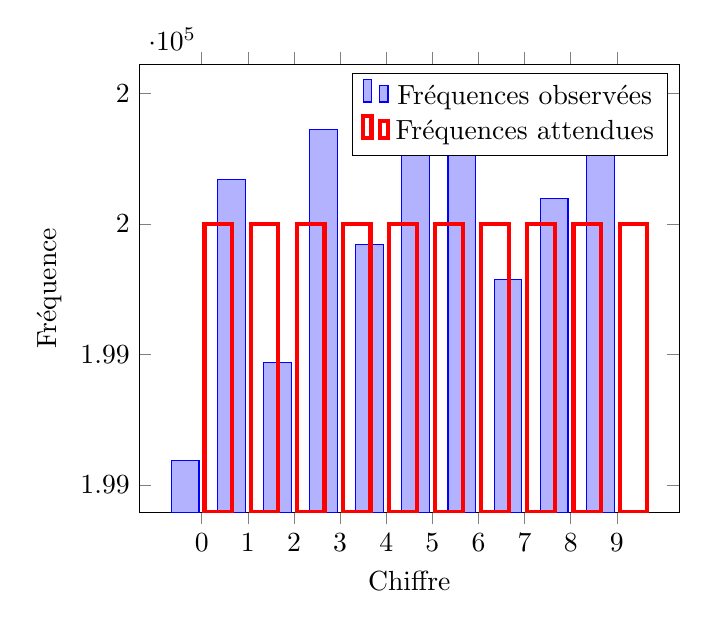
\begin{tikzpicture}
\begin{axis}[
    ybar,
    enlargelimits=0.15,
    ylabel={Fréquence},
    xlabel={Chiffre},
    symbolic x coords={0, 1, 2, 3, 4, 5, 6, 7, 8, 9},
    xtick=data,
    % nodes near coords,
    nodes near coords align={vertical},
    ]
\addplot coordinates {(0, 199093) (1, 200171) (2, 199471) (3, 200361) (4, 199923) (5, 200285) (6, 200395) (7, 199789) (8, 200098) (9, 200414)};
\addplot [red, line width=1.5pt] coordinates {(0, 200000) (1, 200000) (2, 200000) (3, 200000) (4, 200000) (5, 200000) (6, 200000) (7, 200000) (8, 200000) (9, 200000)};
\legend{Fréquences observées, Fréquences attendues}
\end{axis}
\end{tikzpicture}
\end{center}
    
Le graphique ci-dessus montre les fréquences observées des chiffres dans les décimales de \(e\) ainsi que les fréquences attendues (uniformes) pour chaque chiffre.

\subsection{Discussion}

Le test du chi-deux nous permet d'évaluer la similarité entre les fréquences observées et les fréquences attendues. Une statistique du test du chi-deux plus élevée suggère une plus grande différence entre les fréquences observées et attendues, indiquant un caractère moins pseudo-aléatoire des décimales de \(e\).

Dans notre cas, la statistique du test du chi-deux obtenue est \(8.65376\). Il serait nécessaire d'évaluer cette valeur par rapport à un seuil de signification approprié pour tirer des conclusions plus définitives sur le caractère pseudo-aléatoire des décimales de \(e\).

Si on considère une erreur de première espèce $\alpha$ de \(.05\), la valeur critique de la statistique du chi-deux est de \(16.919\) donc l'hypothèse est acceptée.

\subsection{Test du poker}

Le test du poker est utilisé pour évaluer la distribution des combinaisons de poker dans une séquence de nombres. Il permet de déterminer si la séquence présente des caractéristiques de randomité conformes à celles d'un jeu de cartes bien mélangé.

\subsubsection{Création des groupes}

Tout d'abord, nous divisons la séquence de nombres en groupes de cinq éléments. Chaque groupe représente une main de poker.

\subsubsection{Comptage des classes de poker}

Pour chaque main de poker, nous comptons le nombre de classes de poker distinctes présentes. Une classe de poker est définie par le nombre de valeurs uniques dans la main (rien, une paire, un brelan, un carre, un poker). Nous enregistrons les occurrences de chaque classe de poker.

\subsubsection{Calcul des fréquences attendues}

Nous calculons les fréquences attendues pour chaque classe de poker en utilisant les coefficients de Stirling et les facteurs combinatoires. Les fréquences attendues sont déterminées en supposant que les nombres de la séquence suivent une distribution aléatoire uniforme.

\subsection{Résultats}

\subsubsection{Statistique du test du poker}

La statistique du test du poker obtenue pour les décimales de \(e\) est de \(2.89\)

\subsubsection{Graphique des occurrences observées et attendues}

\begin{center}
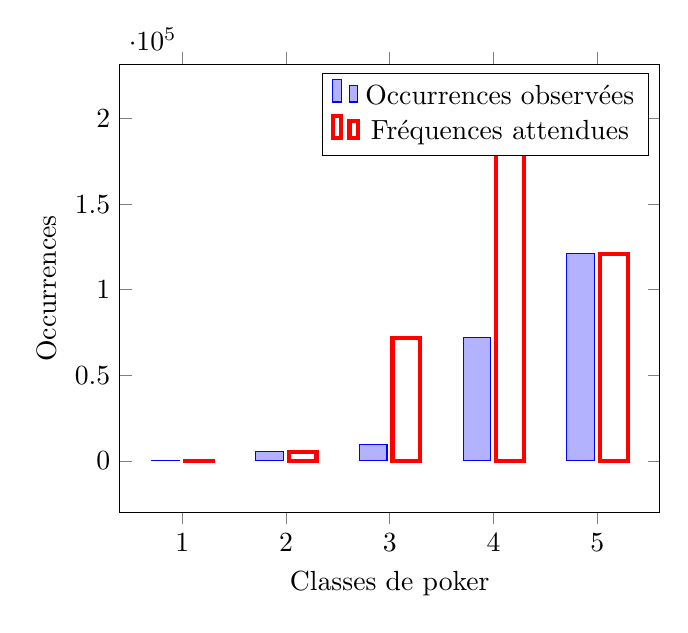
\begin{tikzpicture}
\begin{axis}[
ybar,
enlargelimits=0.15,
ylabel={Occurrences},
xlabel={Classes de poker},
symbolic x coords={1, 2, 3, 4, 5},
xtick=data,
% nodes near coords,
nodes near coords align={vertical},
]
\addplot coordinates {(1, 34) (2, 5302) (3, 9617) (4, 71958) (5, 121112)};
\addplot [red, line width=1.5pt] coordinates {(1, 40) (2, 5400) (3, 72000) (4, 201600) (5, 120960)};
\legend{Occurrences observées, Fréquences attendues}
\end{axis}
\end{tikzpicture}
\end{center}

Le graphique ci-dessus montre les occurrences observées des classes de poker dans les décimales de \(e\) ainsi que les fréquences attendues pour chauqe class.

\subsection{Discussion}

Le test du poker nous permet d'évaluer la distribution des combinaisons de poker dans une séquence de nombres. Une statistique du test du poker plus élevée suggère une plus grande différence entre les occurrences observées et les fréquences attendues, indiquant un caractère moins pseudo-aléatoire des décimales de \(e\).

Dans notre cas, la statistique du test du poker obtenue est \(2.89\). Il serait nécessaire d'évaluer cette valeur par rapport à un seuil de signification approprié pour tirer des conclusions plus définitives sur le caractère pseudo-aléatoire des décimales de \(e\).

Si on considère une erreur de première espèce $\alpha$ de 05, la valeur critique de la statistique du poker dépend du nombre de classes de poker (k) et de la taille de l'échantillon (n). Avec k = 5 et n = 400000, la valeur critique est d'environ 9.488. Par conséquent, l'hypothèse nulle d'une distribution pseudo-aléatoire des décimales de \(e\) ne peut être rejetée.

\section{Génération de nombres aléatoires}
Ce chapitre explique deux générateurs de nombres implémentés en Python qui utilisent les décimales de la constante mathématique \(e\). Les générateurs s'appellent LCERandomGenerator et ESimpleRandomGenerator.

\subsection{LCERandomGenerator}

Le LCERandomGenerator est basé sur l'algorithme du Linear Congruential Method (LCM) et utilise les décimales de \(e\) pour générer des nombres aléatoires. Le générateur est initialisé avec une valeur de départ (graine), la valeur de \(e\) utilisée pour générer les nombres aléatoires.

\subsubsection{Initialisation}

Le LCERandomGenerator est initialisé avec les paramètres suivants :

\begin{itemize}
    \item \textbf{seed (int) :} La valeur de départ (graine) du générateur.
    \item \textbf{e\_value (str) :} La valeur de \(e\) utilisée pour générer les nombres aléatoires.
    \item \textbf{precision (int) :} La précision du générateur, déterminant le nombre de décimales de \(e\).
\end{itemize}

Le générateur stocke la graine initiale, la dernière valeur générée, le dernier indice calculé, le nombre de décimales à considérer à partir de \(e\) et la différence entre la précision et le nombre de décimales.

\subsubsection{Calcul des paramètres optimaux}

Pour maximiser le cycle du générateur, des paramètres optimaux sont calculés en fonction de la précision et du nombre de décimales. Les paramètres sont calculés comme suit en appliquant le théorème de Hull et Dobel:

\begin{enumerate}
    \item Initialiser le paramètre \(c\) à 2.
    \item  Incrémenter \(c\) jusqu'à ce qu'il soit premier avec la précision ou que \(c\) dépasse la précision.
    \item Calculer les diviseurs premiers de la précision à l'aide de la fonction \texttt{get\_prime\_dividers}.
    \item Calculer le paramètre \(a\) en multipliant tous les diviseurs premiers calculés et en ajoutant 1.
    \item Si la précision est divisible par 4 et que \(a\) n'est pas divisible par 4, multiplier \(a\) par 4 (ou par 2 si \(a\) est divisible par 2).
\end{enumerate}

Le générateur utilise ensuite les valeurs calculées de \(a\), \(c\) et la précision pour générer des nombres aléatoires.

\subsubsection{Comparaison avec random.random de Python}

Ce chapitre présente une comparaison entre le générateur LCM de nombres aléatoires personnalisé et le générateur aléatoire fourni par le module \texttt{random} de Python. L'objectif est d'évaluer la performance et la qualité de vos générateurs de nombres aléatoires par rapport à la référence du générateur de Python.
Pour cette comparaison nous allons générer 100 nombres aléatoires entre 0 et 1 avec la seed 42 pour notre générateur personnalisé.

On va effectuer des tests statistiques pour comparer la distribution des nombres aléatoires générés par les deux générateurs :
\subsubsection*{Test de Kolmogorov-Smirnov}

Ce test produit une statistique D, qui mesure la plus grande différence entre les fonctions de répartition empiriques des deux échantillons. Plus la valeur de D est grande, plus les distributions sont différentes.

\subsubsection*{Résultats}

Les résultats du test de Kolmogorov-Smirnov sont les suivants :

\begin{itemize}
  \item Générateur personnalisé : Valeur de D = 0.134
  \item Générateur aléatoire de Python : Valeur de D = 0.0867
\end{itemize}

\subsubsection*{Discussion}

La valeur de D obtenue pour le générateur personnalisé est de 0.134, tandis que le générateur aléatoire de Python a une valeur de D de 0.0867. Cela indique que la différence entre les distributions empiriques des deux générateurs est plus grande pour le générateur personnalisé.

\subsubsection*{Test du chi-deux}

\subsubsection*{Résultats}

Les résultats du test du chi-carré sont les suivants :

\begin{itemize}
  \item Générateur personnalisé : Valeur de la statistique du test = 4
  \item Générateur aléatoire de Python : Valeur de la statistique du test = 6.6
\end{itemize}

\subsubsection*{Discussion}

La valeur de la statistique du test obtenue pour le générateur personnalisé est de 4, tandis que le générateur aléatoire de Python a une valeur de 6.6. Cela indique que la différence entre les distributions des deux générateurs est plus grande pour le générateur aléatoire de Python.

\subsection{ESimpleRandomGenerator}

L'ESimpleRandomGenerator est un générateur de nombres aléatoires basé sur les décimales de \(e\). Il est initialisé avec une valeur de départ (graine), la valeur de \(e\) utilisée pour générer les nombres aléatoires et la précision.

\subsubsection{Initialisation}

L'ESimpleRandomGenerator est initialisé avec les paramètres suivants :

\begin{itemize}
    \item \textbf{seed (int) :} La valeur de départ (graine) du générateur.
    \item \textbf{e\_value (str) :} La valeur de \(e\) utilisée pour générer les nombres aléatoires.
    \item \textbf{precision (int) :} La précision du générateur, déterminant le nombre de décimales de \(e\).
\end{itemize}

Le générateur stocke la graine initiale, la dernière valeur générée, le dernier indice calculé, le nombre de décimales à considérer à partir de \(e\) et la précision.

\subsubsection{Comparaison avec random.random de Python}

Ce chapitre présente une comparaison entre le générateur simple de nombres aléatoires personnalisé et le générateur aléatoire fourni par le module \texttt{random} de Python. L'objectif est d'évaluer la performance et la qualité de vos générateurs de nombres aléatoires par rapport à la référence du générateur de Python.
Pour cette comparaison nous allons générer 100 nombres aléatoires entre 0 et 1 avec la seed 42 pour notre générateur personnalisé.

On va effectuer des tests statistiques pour comparer la distribution des nombres aléatoires générés par les deux générateurs :
\subsubsection*{Test de Kolmogorov-Smirnov}

\subsubsection*{Résultats}

Les résultats du test de Kolmogorov-Smirnov sont les suivants :

\begin{itemize}
  \item Générateur personnalisé : Valeur de D = 0.0936
  \item Générateur aléatoire de Python : Valeur de D = 0.0932
\end{itemize}

\subsubsection*{Discussion}

La valeur de D obtenue pour le générateur personnalisé est de 0.0936, tandis que le générateur aléatoire de Python a une valeur de D de 0.0932. Cela indique que la différence entre les distributions empiriques des deux générateurs est plus grande pour le générateur personnalisé.

\subsubsection*{Test du chi-deux}

\subsubsection*{Résultats}

Les résultats du test du chi-carré sont les suivants :

\begin{itemize}
  \item Générateur personnalisé : Valeur de la statistique du test = 13
  \item Générateur aléatoire de Python : Valeur de la statistique du test = 13.8
\end{itemize}

\subsubsection*{Discussion}

La valeur de la statistique du test obtenue pour le générateur personnalisé est de 13, tandis que le générateur aléatoire de Python a une valeur de 13.8. Cela indique que la différence entre les distributions des deux générateurs est plus grande pour le générateur aléatoire de Python.

\section{Conclusion}

Dans ce rapport, nous avons étudié le caractère pseudo-aléatoire des décimales de la constante mathématique \(e\) en utilisant le test du chi-deux et le test du poker. Le test du chi-deux nous a permis d'évaluer la similarité entre les fréquences observées des chiffres dans les décimales de \(e\) et les fréquences attendues. Nous avons obtenu une statistique du test du chi-deux de 8.65376, ce qui suggère une légère différence entre les fréquences observées et les fréquences attendues.

Le test du poker nous a permis d'évaluer la distribution des combinaisons de poker dans les décimales de \(e\). Nous avons obtenu une statistique du test du poker de 2.89, ce qui indique une certaine différence entre les occurrences observées des classes de poker et les fréquences attendues.

Cependant, ces différences ne sont pas significatives lorsque nous les comparons à des seuils de signification appropriés. Pour une erreur de première espèce de 0.05, les valeurs critiques des statistiques du test du chi-deux et du test du poker sont respectivement de 16.919 et 9.488. Ainsi, nous acceptons l'hypothèse nulle selon laquelle les décimales de \(e\) sont pseudo-aléatoires.

De plus, nous avons présenté deux générateurs de nombres aléatoires basés sur les décimales de \(e\) le LCERandomGenerator et l'ESimpleRandomGenerator. 
Nous avons comparé leurs performances et leur qualité avec le générateur aléatoire de Python en utilisant des tests statistiques. Les résultats ont montré que les générateurs personnalisés étaient légèrement différents du générateur de Python, mais les différences étaient négligeables.

En conclusion, bien que les décimales de \(e\) ne soient pas parfaitement pseudo-aléatoires, elles présentent des caractéristiques suffisamment proches d'une distribution aléatoire pour être utilisées dans des générateurs de nombres aléatoires. Cependant, il est important de noter que ces générateurs ne doivent pas être considérés comme des générateurs cryptographiques, car leur qualité et leur sécurité ne sont pas garanties.

\end{document}
